\documentclass[tikz]{standalone}
\tikzset{
	source/.pic = {
		\draw (0.5, 0.7) -- ++(0, -0.2) --
		      ++(-0.5, 0) -- ++(0, 0.5) --
		      ++(-0.7, 0) -- ++(0, -2) --
		      ++(0.7, 0) -- ++(0, 0.5) --
		      ++(0.5, 0) -- ++(0, -0.2);
	},
	detector/.pic = {
		\draw [fill=gray] (-1, 1) rectangle (1, -1);
		\draw (-0.8, 1) -- ++(0, -2);
	},
	slab/.pic = {
		\draw [fill=gray!50] (-0.2, 2) rectangle (0.2, -2);
	},
	human/.pic = {
		\draw [fill=gray] (0, 0) 
		.. controls ++(180:-1) and ++(-90: 1) .. ( 2, 1)
		.. controls ++(-90:-1) and ++(180:-1) .. ( 0, 2)
		.. controls ++(180: 1) and ++(-90:-1) .. (-2, 1)
		.. controls ++(-90: 1) and ++(180: 1) .. ( 0, 0);
		\draw [fill=white] (0, 1.5) ellipse (0.8 and 1);
		\draw (-.1, 2.49) to [in=180, out=30] ++(0.1, 0.2) to [in=150, out=0] ++(0.1, -0.2);
		\path[thick, fill=white] (-.1, 2.48) to [in=180, out=30] ++(0.1, 0.2) to [in=150, out=0] ++(0.1, -0.2) --cycle;
	}
}


\begin{document}
	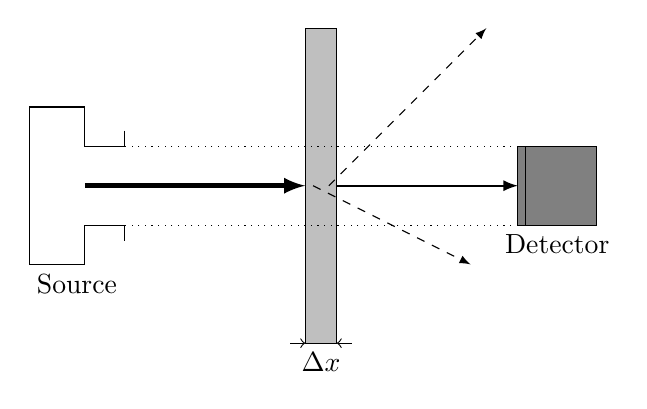
\begin{tikzpicture}
		\pic [local bounding box=source]  at (-3, 0) {source};
		\node [below] at (source.south) {Source};
		\pic [scale=0.5, local bounding box=detector] at (3, 0) {detector};
		\node [below] at (detector.south) {Detector};
		\pic [local bounding box=slab] at (0, 0) {slab};
		\draw [ultra thick, -latex] (-3, 0) -- (slab.west);
		\draw [thick, -latex] (slab.east) -- (detector.west);
		\node [below] at (slab.south) {\( \Delta x \)};
		\draw [dotted] (detector.north west) -- (detector.north -| source.east);
		\draw [dotted] (detector.south west) -- (detector.south -| source.east);
		\draw [<-] (slab.south west) -- ++(-0.2, 0);
		\draw [<-] (slab.south east) -- ++(0.2, 0);
		\draw [dashed, -latex] (0.1, 0.) -- ++(2, 2);
		\draw [dashed, -latex] (-0.1, 0.) -- ++(2, -1);
	\end{tikzpicture}
\end{document}
